\documentclass[11pt]{report}
\usepackage{graphicx}
\usepackage{float}
\title{EE314 Experiment 3 Parallel Adders, Subtractors and Complementors}
\date{2018\\ March}
\author{Nail Tosun - 2094563\\ Electric and Electronic Engineering Departmant, METU}
\begin{document}
\maketitle
2)
\begin{figure}[H]
  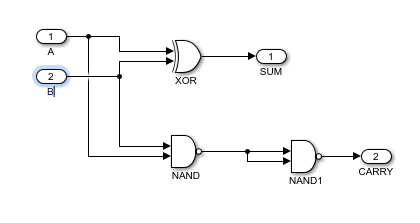
\includegraphics[width=\linewidth]{halfadder}
  \caption{Half-adder circuit using NAND and XOR gates}
  \label{fig:zero}
\end{figure} 

\begin{table}[H]
\centering
\caption{Truth table of half adder}
\label{my-label}
\begin{tabular}{cccc}
A & B & C & S \\
0 & 0 & 0 & 0 \\
0 & 1 & 0 & 1 \\
1 & 0 & 0 & 1 \\
1 & 1 & 1 & 0
\end{tabular}
\end{table}

\begin{figure}[H]
  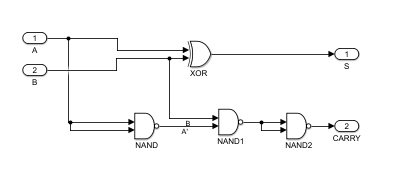
\includegraphics[width=\linewidth]{halfsub}
  \caption{Half-subtractor consists of NAND and XOR}
  \label{fig:zero}
\end{figure}

\begin{table}[H]
\centering
\caption{Truth table of half subtractor}
\label{my-label}
\begin{tabular}{cccc}
A & B & CARRY & S \\
0 & 0 & 0 & 0 \\
0 & 1 & 1 & 1 \\
1 & 0 & 0 & 1 \\
1 & 1 & 0 & 0
\end{tabular}
\end{table}

\begin{figure}[H]
  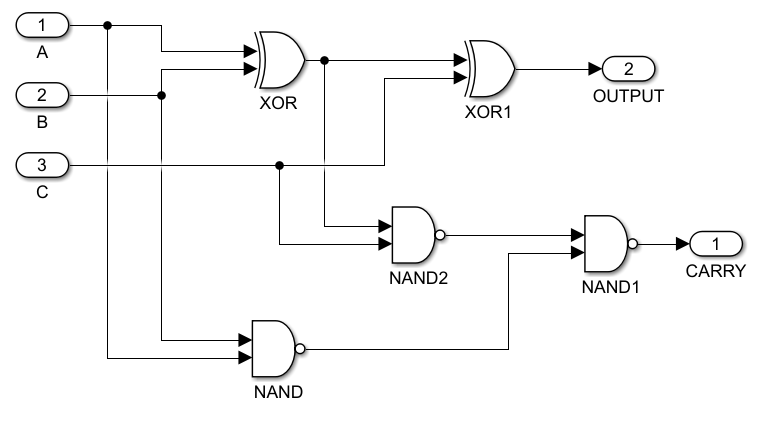
\includegraphics[width=\linewidth]{fulladder}
  \caption{Full-adder circuit using NAND and XOR gates}
  \label{fig:zero}
\end{figure}
\begin{table}[H]
\centering
\caption{Full-adder truth table}
\label{my-label}
\begin{tabular}{ccccl}
A                     & B                     & C                     & Carry & Sum \\
0                     & 0                     & 0                     & 0     & 0   \\
0                     & 0                     & 1                     & 0     & 1   \\
0                     & 1                     & 0                     & 0     & 1   \\
0                     & 1                     & 1                     & 1     & 0   \\
\multicolumn{1}{l}{1} & \multicolumn{1}{l}{0} & \multicolumn{1}{l}{0} & 0     & 1   \\
1                     & 0                     & 1                     & 1     & 0   \\
1                     & 1                     & 0                     & 1     & 0   \\
1                     & 1                     & 1                     & 1     & 1  
\end{tabular}
\end{table}
\begin{figure}[H]
  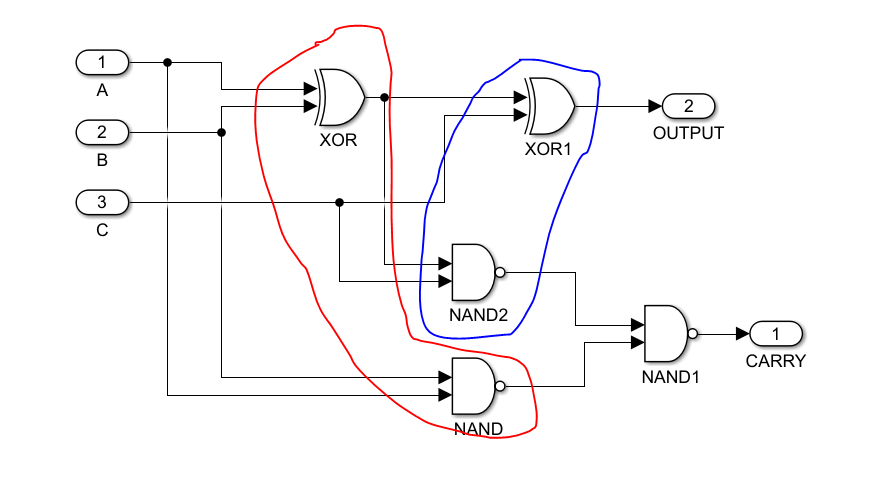
\includegraphics[width=\linewidth]{fulladder1}
  \caption{Full adder consists of two half adder}
  \label{fig:zero}
\end{figure}

4)
\begin{figure}[H]
  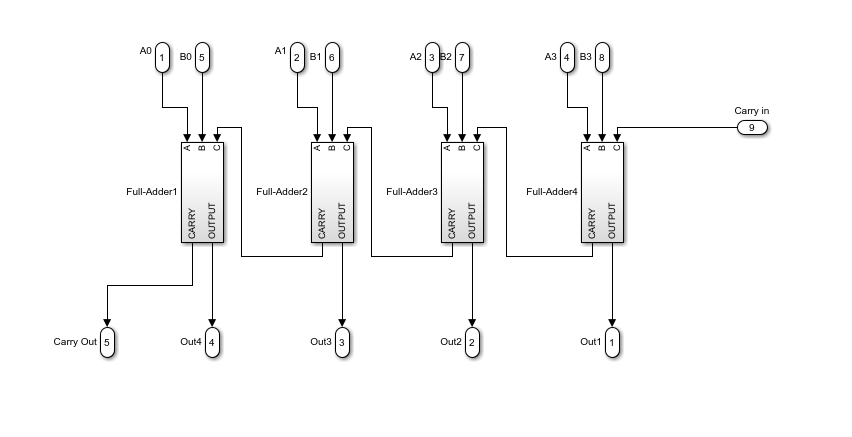
\includegraphics[width=\linewidth]{fourbitadder}
  \caption{Four bit adder using full adders using Simulink (I)}
  \label{fig:zero}
\end{figure}

6)
\begin{figure}[H]
  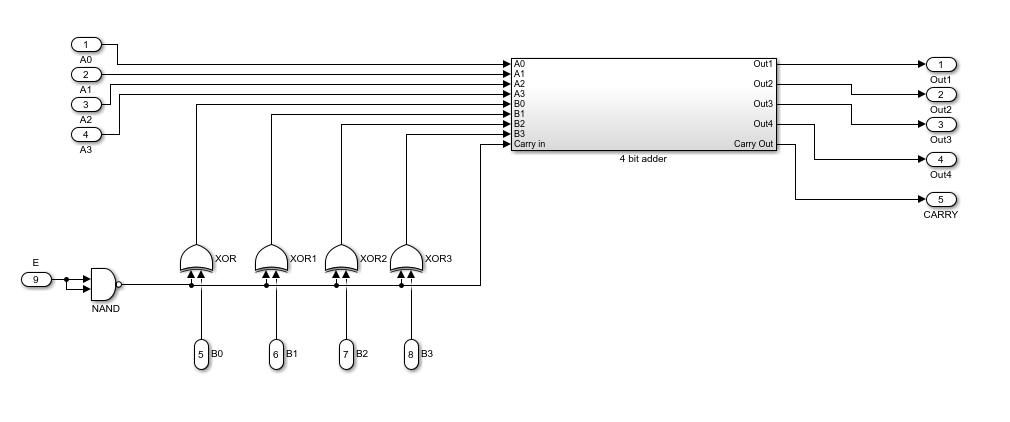
\includegraphics[width=\linewidth]{design}
  \caption{Four bit adder and substractor using 2's complement technique with enable pin using Simulink (I)}
  \label{fig:zero}
\end{figure}

7)
\begin{table}[]
\centering
\caption{Truth table}
\label{my-label}
\begin{tabular}{ccccl}
E                     & X                        & Y                        & OUT     & CARRY   \\
1                     & 0110                     & 0011                     & 1001    & 0       \\
1                     & 0111                     & 0001                     & 1000    & 0       \\
0                     & 0110                     & 0001                     & 0101    & 0       \\
0                     & 0011                     & 0100                     & 1111    & 0       \\
\multicolumn{1}{l}{1} & \multicolumn{1}{l}{1010} & \multicolumn{1}{l}{0111} & 0001    & 1       \\
1                     & 1011                     & invalid                  & invalid & invalid \\
0                     & 1001                     & 0110                     & 0011    & 1       \\
0                     & 1111                     & invalid                  & invalid & invalid
\end{tabular}
\end{table}

References and Notes:
(I) If figure is not clear original document can found by following URL.

8)
 \begin{figure}[H]
  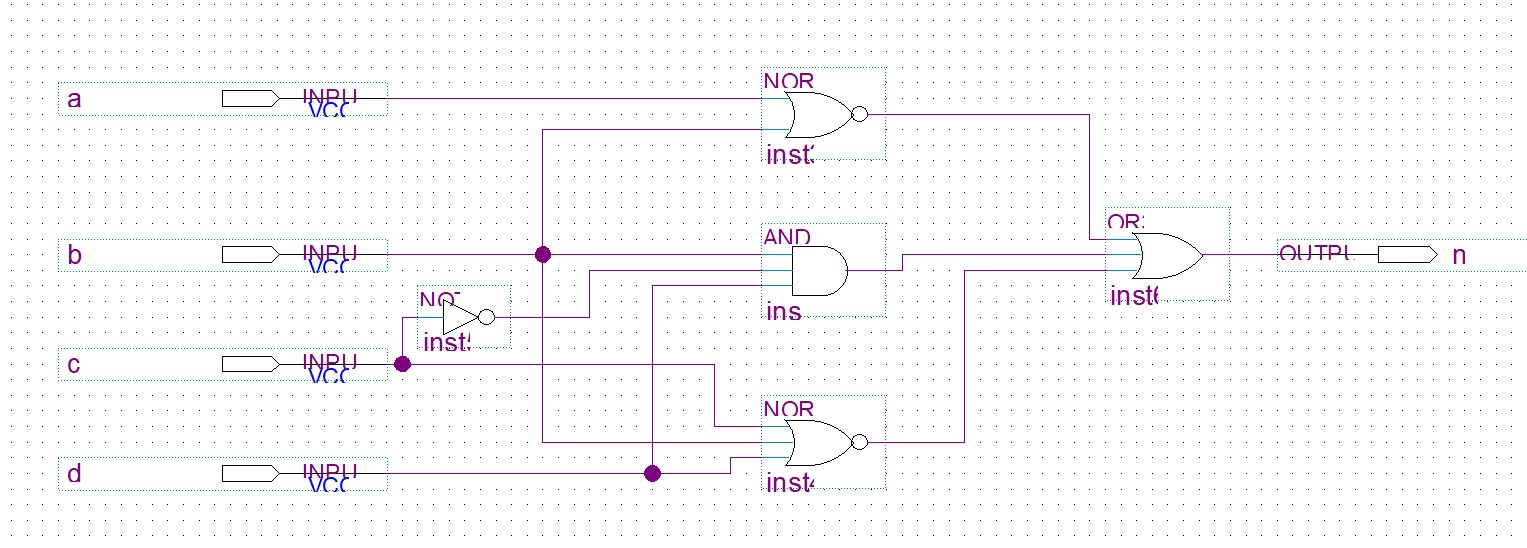
\includegraphics[width=\linewidth]{bos}
  \caption{ }
  \label{fig:zero}
\end{figure}

 \begin{figure}[H]
  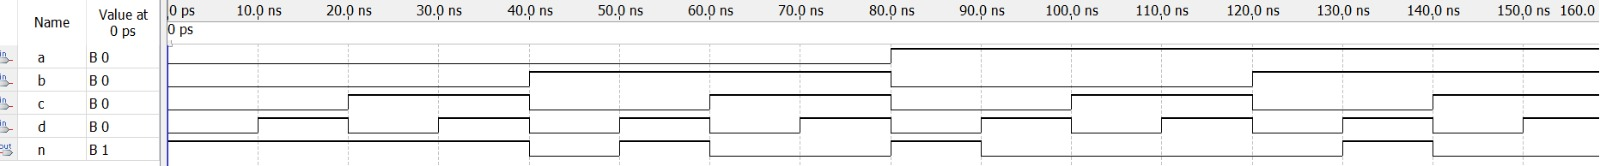
\includegraphics[width=\linewidth]{boos}
  \caption{ }
  \label{fig:zero}
\end{figure}
 \begin{figure}[H]
  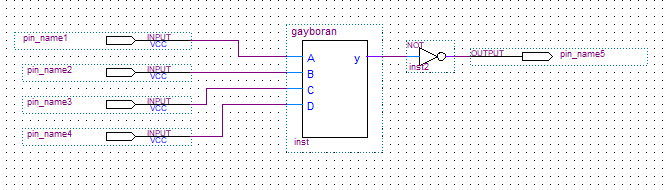
\includegraphics[width=\linewidth]{sim}
  \caption{ }
  \label{fig:zero}
\end{figure}
 \begin{figure}[H]
  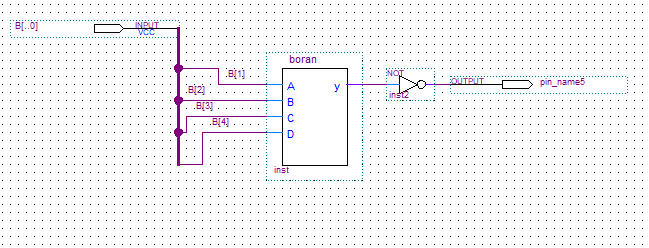
\includegraphics[width=\linewidth]{boran}
  \caption{ }
  \label{fig:zero}
\end{figure}
Since i have problem with Quartus simulation results didn't work.

\end{document}